\section{Computer architecture from a performance point of view: from serial to parallel} 


The goal of this section is to introduce key concepts of computer architecture in order to: 
\begin{itemize}
    \item[-] Identify the characteristics of the processors that most influence the computing performance;
    \item[-] Identify the limits of the standard architecture (Dennard and Moore scaling, Flynn's taxonomy);
    \item[-] Introduce concurrency and parallelism and study their limits (Amdahl and Gustafson laws).
\end{itemize} 

\subsection{Von Neumann architecture}
The so-called \textbf{Von Neumann architecture} was introduced in 1945 by John von Neumann and is based on the \textit{Universal Turing Machine} (UTM) by Alan Turing (1936). It consists of 5 main elements:

\begin{center}
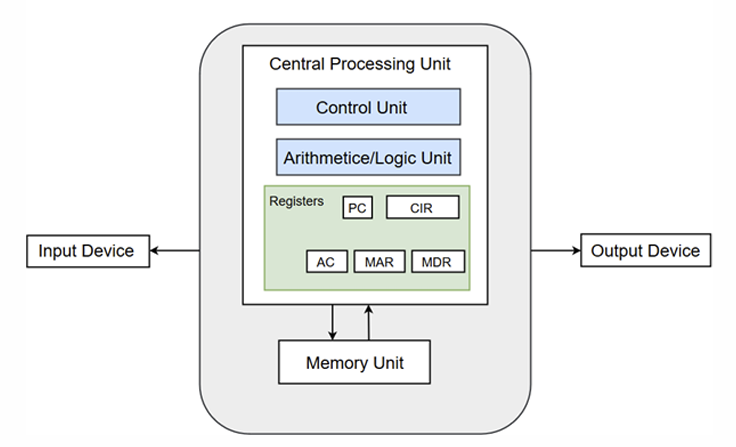
\includegraphics[width=0.6\textwidth]{figuresP/lesson_parallel_1_pag_6.png}
\end{center}

\begin{itemize}
    \item \textbf{Central Processing Unit} (CPU) composed of:
    \begin{itemize}
    \item \textbf{Arithmetic and Logic Unit (ALU)}: performs all arithmetic calculations and logical operations required to execute instructions.
    \item \textbf{Control Unit}: decodes instructions fetched from memory and orchestrates the operation of the entire system by sending timing and control signals.
    \end{itemize}
    \item \textbf{Memory}: a shared storage area that holds both the program's instructions and the data currently being processed. The so-called \textbf{Random Access Memory (RAM)} is the \textit{primary memory}. It is volatile (data is lost when power is cut) and it is the one that actually stores the instructions and data of currently running processes. The \textbf{Secondary Storage (SSD/HDD)} commonly referred to as "disk space,"  is the \textit{non-volatile} storage. It is designed for long-term data retention. While significantly slower than RAM, it offers much larger capacities at a lower cost. Finally, the CPU itself has local, fast-read memory units called \textbf{registers}. 
    \item \textbf{Bus}: communication system composed of physical wires that transfers addresses, data, and signals between the CPU, memory, and peripherals.
    \item \textbf{I/O (Input/Output)}: interfaces that allow the computer to interact with the external world, receiving data from users and providing the results of computations.
\end{itemize}

The so-called \textbf{Von Neumann bottleneck} refers to the throughput limitation between the CPU and memory, which occurs because the shared bus cannot fetch instructions and data simultaneously. To mitigate this phenomenon and improve performance, several hardware strategies are employed:
\begin{itemize}
    \item \textbf{Caching and Memory Hierarchy}: Small, high-speed memory units (L1, L2, L3 \textbf{caches}) are placed directly on the CPU chip to store frequently used data and instructions, drastically reducing the number of slow accesses to the main RAM. A multilevel cache represents a good trade-off between hit-rate and latency. For example the \textbf{I-Cache} and \textbf{D-Cache} are L1 caches dedicated respectively to instructions and data to avoid access conflicts at the core level. The hierarchy of both data access and instruction fetching is fundamental in present computer architecture.
    \begin{center}
        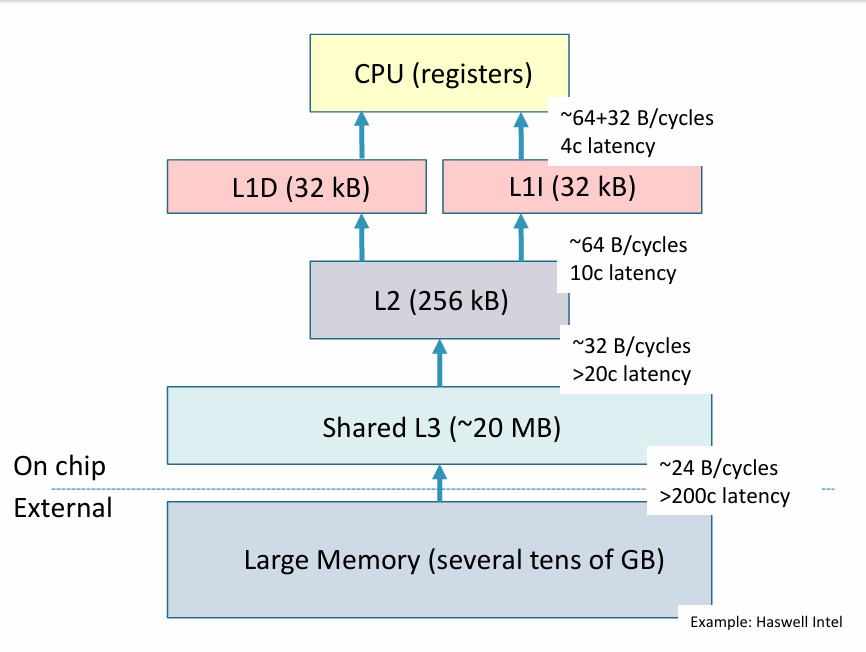
\includegraphics[width=0.6\textwidth]{figuresP/lesson_parallel_1_pag_9.png}   
    \end{center}
    \item \textbf{Harvard Architecture}: By providing separate physical pathways and storage for instructions and data, the processor can perform an instruction fetch and a data access at the same time, effectively doubling the available bandwidth (see representation below).
    \begin{center}
        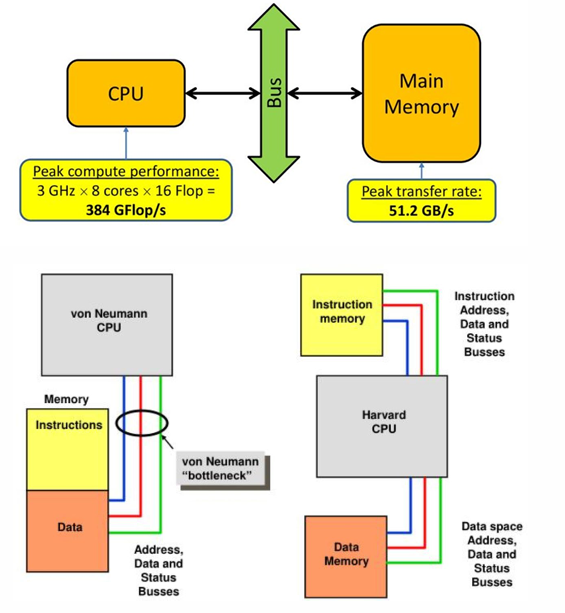
\includegraphics[width=0.4\textwidth]{figuresP/lesson_parallel_1_pag_7.png}
    \end{center}
    \item \textbf{Branch Prediction}: A sophisticated technique where the CPU "guesses" the outcome of conditional statements (e.g., \texttt{if} blocks) to pre-fetch and begin executing the most likely next instructions, preventing the pipeline from stalling (see below).
\end{itemize}

\hrulefill

\subsubsection{Note: simple server architecture}

A \textbf{server} is a specialized computer system or a software process designed to provide services, data, or resources to other programs or devices, known as \textbf{clients}, over a network. This interaction follows the \textbf{client-server model}, where the server "listens" for incoming requests and responds by processing the required task or delivering the requested information.

From a hardware perspective, servers are typically high-performance machines engineered for reliability and availability, often operating 24/7. From a software perspective, a server is a program (such as a web server or a database server) that manages access to a centralized resource. \footnote{The previous definition of a server was surely NOT given by ChatGPT}.

In a modern server, several components interact to execute programs efficiently:
\begin{itemize}
    \item[-] \textit{Processors/Cores}: Processing units that execute instructions, often organized in multi-core layouts for parallel computation.
    \item[-] \textit{Shared Caches (L3)}: A larger memory pool shared among all cores to synchronize data and minimize slow accesses to the main RAM.
    \item[-] \textit{Memory Controllers}: Logic circuits that manage the high-speed data flow between the processor and the system memory.
    \item[-] \textit{I/O Subsystems}: The infrastructure (e.g., PCIe) connecting the CPU to storage, network, and external peripherals.
\end{itemize}
For example \textit{NUMA (Non-Uniform Memory Access)} is a multi-socket architecture where memory access latency depends on the physical distance between the processor and the memory bank.

\begin{center}
    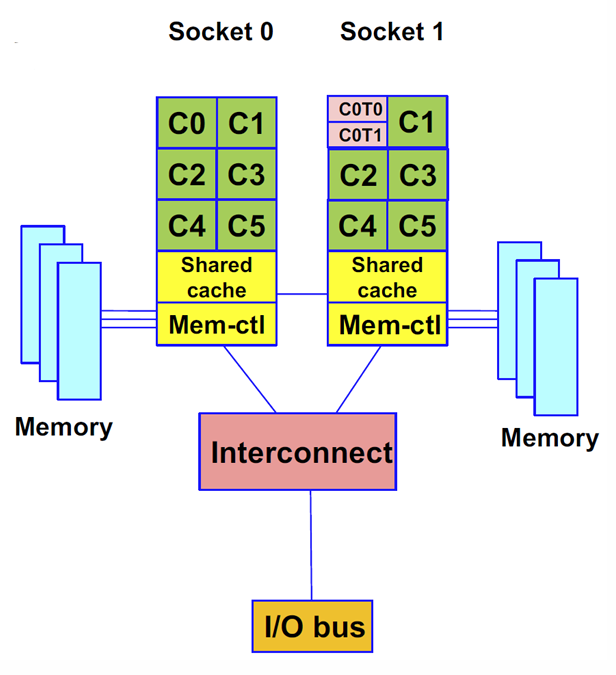
\includegraphics[width=0.4\textwidth]{figuresP/lesson_parallel_1_pag_8.png}
\end{center}

\hrulefill

\subsection{Parallelism and the seven dimensions of performance}
The modern PC performance depends on (at least) seven characteristics:
\begin{itemize}
    \item[-] Data and Instruction level:
    \begin{itemize}
        \item[1] Hardware vectors
        \item[2] Superscalars
        \item[3] Pipelining
    \end{itemize}
    \item[-] Task level:
    \begin{itemize}
        \item[4] Hardware multithreading
        \item[5] Multiple cores
        \item[6] Multiple sockets
    \end{itemize}
    \item[-] Application level: 
    \begin{itemize}
        \item[7] Multiple nodes
    \end{itemize}
\end{itemize}
Obviously, our goal is to maximize the performance of our PC, which means reducing the execution time of our program. In other words, we want to complete a certain task in the least possible amount of clock cycles. The best way to do it is \textit{parallelism}.

\textbf{Parallelism} is the simultaneous execution of multiple computations. While often associated with multi-core processors, parallelism actually occurs at different "dimensions", matching the "levels" listed above. 

It starts at the micro level with \textbf{Instruction Level Parallelism (ILP)}, where a single core overlaps the execution of machine instructions. It scales up to \textbf{Task Level Parallelism (TLP)}, where distinct \textit{threads} or processes run on separate physical cores or processors. Remember this definition: a \textbf{thread} is the smallest instruction set that can be managed independently by a scheduler (typically in the operating system). Finally, it reaches the \textbf{Application Level}, where workloads are distributed across entirely different machines (nodes).

We will now dive a little deeper into the first 3 points of the "performance list", but the next 4 will be the central core of this part of the course. 

\hrulefill

\subsubsection{Note: Clock Cycles}
A \textbf{clock cycle} is the fundamental unit of time for a processor, acting as an electronic "heartbeat" that synchronizes internal operations. The \textit{clock rate} (frequency), measured in Gigahertz (GHz), defines how many billions of cycles occur per second. While a higher frequency generally speeds up execution by shortening the interval between processing steps, the actual performance also depends on the \textit{CPI} (Cycles Per Instruction). Since different instructions require a varying number of cycles to complete, true execution speed is a trade-off between how fast the clock "ticks" and how efficiently instructions are retired during each cycle.

\hrulefill

\subsection{Instruction level parallelism}
\subsubsection{[1] Vector processors}
Modern processors incorporate specialized hardware and wide registers (such as XMM and YMM) to support hardware-level \textbf{vectorization} through instruction sets like \textbf{SSE/SSE2} and \textbf{AVX}. You probably don't know what these are, but just remember that when you work with \texttt{numpy} arrays you are exploiting them without even knowing it. With these components, one can obtain a \textit{SIMD (Single Instruction Multiple Data)} architecture (one operation produces multiple results, e.g. a sum of two vectors of 4 floating point elements is a single instruction that produces 4 results) even in a single core. We will get to this concept in a second. \\
Vectorization at the instruction level is the first simple example of parallelism. 

\begin{center}
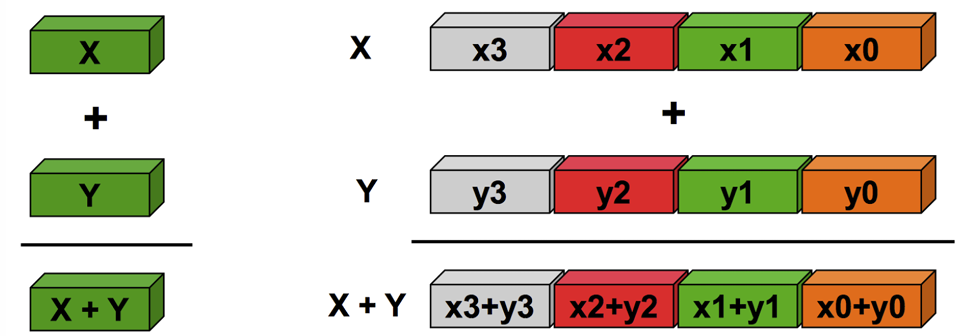
\includegraphics[width=0.4\textwidth]{figuresP/lesson_parallel_1_pag_11.png}
\end{center}

\subsubsection{[2] Superscalars}
A \textbf{superscalar} architecture is in between pure scalar and pure vector. In the CPU there can be several hardware units called \textbf{Functional Units (FU)} that can execute different operations on different data at the same time and can be "specialized" for certain tasks. A \textit{decoder} "reads" the incoming instruction stream and passes it to the \textit{dispatcher}, which assigns the correct task to each FU. The decoder and the dispatcher must have the capability to manage two instructions in one clock cycle. 

A superscalar processor is useful for \textbf{branch prediction}. To understand this concept, just think about an \texttt{if - else} statement that depends on a certain \texttt{condition}. Before executing one of the two branches of the statement, the CPU must know if \texttt{condition} is \texttt{True} (in which case it will execute the \texttt{if} branch) or \texttt{False} (in which case it will execute the \texttt{else} branch). However, in a superscalar processor two different FUs can simultaneously execute the two branches and then the CPU will choose which one to use once \texttt{condition} is defined. That's a simple example of branch prediction.

\begin{center}
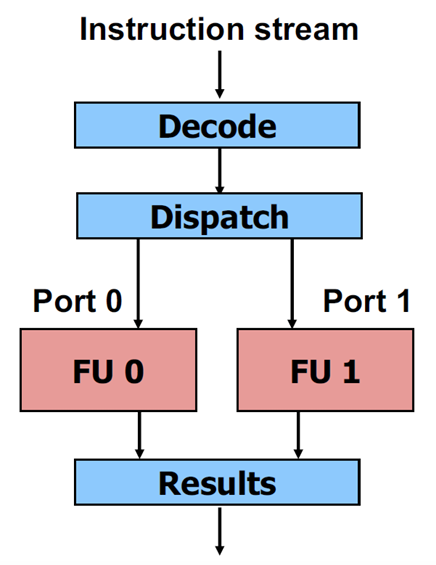
\includegraphics[width=0.3\textwidth]{figuresP/lesson_parallel_1_pag_12.png}
\end{center}

\subsubsection{[3] Pipelining}
What steps does the processor follow to execute an instruction? Here they are:
\begin{itemize}
    \item[-] \underline{Instruction fetching (IF)}: the instructions to execute and the necessary data are fetched from the memory (RAM or cache) thanks to the PC;
    \item[-] \underline{Instruction Decode (ID)}: the processor interprets the instruction and reads the data from the registers;
    \item[-] \underline{Execution (EX)}: the ALU executes the instructions;
    \item[-] \underline{Memory Access (MEM}, done only if the instruction requires to load or store something in the memory);
    \item[-] \underline{Write Back (WB)}: the result is written in a register.
\end{itemize}

Integer and logic instructions have a determined latency, i.e. a fixed number of clock cycles needed for the EX phase. Here are some examples \footnote{You can easily find what these three-letter formulas mean online. "ADD" stands for "addition" (the sum between two integers); "IMUL" is the sum of two floating point numbers etc\dots}: 
\begin{itemize}
    \item[-] 1 cycle: ADD, AND, SHL, ROR, FABS
    \item[-] 3 cycles: IMUL, FADD
    \item[-] 5 cycles: FMUL
    \item[-] 13-23 cycles: IDEV
    \item[-] 27 cycles: FSQRT
\end{itemize} 

\textbf{Pipelining} is the capability to execute different stages of consecutive instructions at the same time. 

Look at the following scheme which represents a pipeline of\textit{ depth 3} (as it "contains" 3 simple operations with 1 cycle for the EX phase): squares vertically aligned contain stages of different instructions that can be executed in the same clock cycle.

Without the pipeline (15 clock cycles of latency):
\begin{center}
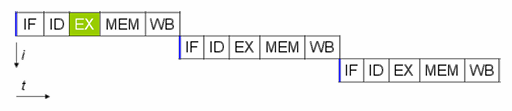
\includegraphics[width=0.7\textwidth]{figuresP/lesson_parallel_1_pag_13.png}
\end{center}

With the pipeline (7 clock cycles of latency):
\begin{center}
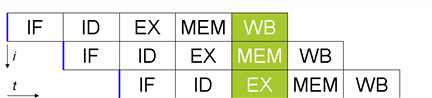
\includegraphics[width=0.6\textwidth]{figuresP/lesson_parallel_1_pag_13a.png}
\end{center}

Here's a more realistic example:
\begin{center}
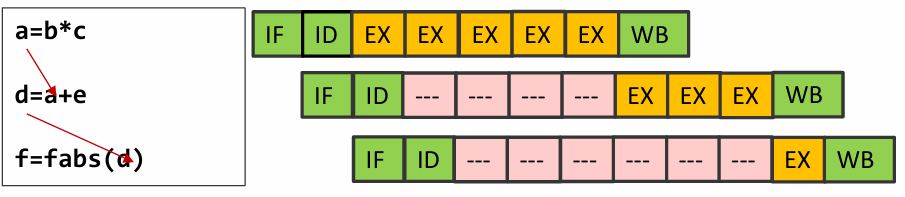
\includegraphics[width=0.9\textwidth]{figuresP/lesson_parallel_1_pag_13b.png}
\end{center}

\subsubsection{Recap and conclusions}
As we've seen, superscalars, pipelining and vectorization are methods to exploit some parallelism at the instruction and data level. Probably \textit{OOO (Out-of-order) execution} should be included in this category, but we won't discuss it here. 

The possible performance improvement thanks to ILP depends on the problem and data structures and can result in $1\times-10\times$ speed-up for superscalars and pipelines and in $2\times, 4\times, 8\times, 16\times$ speed-up for vectorization.

However, these methods will incur in \textit{saturation} because they are limited by the available CPU resources. Here are some examples:
\begin{itemize}
    \item[-] Pentium 4: 30 pipeline stages (nowadays 10-15 maximum), maximum number of pipelines in a processor (2000s).
    \item[-] ARM A57 (Apple A7/A8): 9 ports, 6 instructions superscalar
    \item[-] Intel Tiger Lake: vector of 512 bits for a subset of AVX512 instructions
\end{itemize}
The point is: \textbf{can CPU resources grow indefinitely?}

\subsection{Dennard scaling}

You might think that to enhance performance one could just maximize the clock rate. Nowadays there exist oscillators that can reach a frequency in the order of the THz, so it seems that the speed-up problem just depends on technical innovation towards faster oscillators. However, there's a fallacy in this kind of reasoning.

As you know from the \textit{Digital Technologies} course, modern digital CPUs are based on \textbf{transistors} (like the one represented below), which can be used as switches\footnote{If you want to easily understand how a CPU works thanks to transistors, take a look at this playlist \url{https://youtube.com/playlist?list=PL9vTTBa7QaQOoMfpP3ztvgyQkPWDPfJez&si=i0Yy-61cQFOv8zpt}, and in particular at this video \url{https://youtu.be/HjneAhCy2N4?si=LX_gNx31aW7GgXWl}}. The time needed to switch from a state to the other depends on the gate length $L$. 

\begin{center}
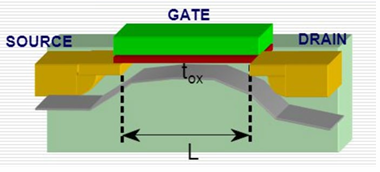
\includegraphics[width=0.45\textwidth]{figuresP/lesson_parallel_1_pag_15.png}
\end{center}

If we are looking for a faster clock cycle, we are then going to need smaller and smaller transistors. In other words, we need more \textbf{integration}, which means that there should be a greater number of components on the same chip surface. In particular the number of transistors that can be integrated on a chip will scale proportionally to $L^2$. However, a larger number of components means a greater consumption of energy to switch the transistors. Is there an energy problem, then? Not really, because the voltage $V$ and the current intensity $i$ needed to switch the transistors scale proportionally to $L$. Since power consumption is equal to $V \cdot i$, the two effects should cancel out. 

The continuous decrease in transistor dimensions ( $\equiv$ increasing integration) is referred to as \textbf{Dennard Scaling} (from an article by Dennard et al. in 1974 in the IEEE Journal of Solid State Circuits). You can find a schematic representation below.

\begin{center}
    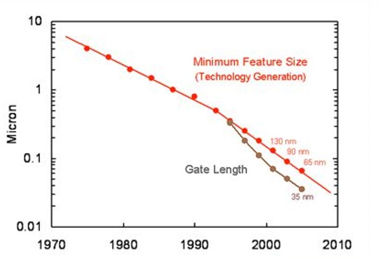
\includegraphics[width=0.49\textwidth]{figuresP/lesson_parallel_1_pag_15a.png}
    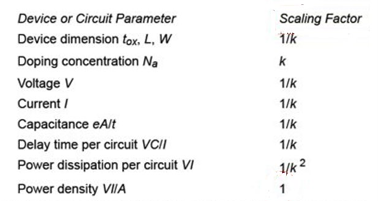
\includegraphics[width=0.49\textwidth]{figuresP/lesson_parallel_1_pag_15b.png}
\end{center}

So\dots what's the matter? With very high integration \textit{it is not true anymore that the power consumption is the same, due to an increase in current leakage}: in smaller transistors you will need more power to compensate for the \textit{inverse currents}. Also, the switching characteristics of a transistor depend on it's temperature, which will rapidly increase in very crowded chips. That means that Dennard scaling cannot continue indefinitely, but processors have a power limit due to heat (even with better packaging and cooling systems).  

\subsection{Moore scaling}
\textbf{Moore's "law"} is the empirical observation that the mean number of transistors per chip doubles about each two years, while the performance of CPU doubles each 18 months. Take a look at the graphs below. \\
Moore's prediction was verified for decades but around 2005 it started to show saturation. That is of course closely related to Dennard scaling. In the first years of the 2000s, people realized that increasing the clock frequency and integrating was not the best way (anymore) to increase the processor performance.

\begin{figure}[H]
    \centering
    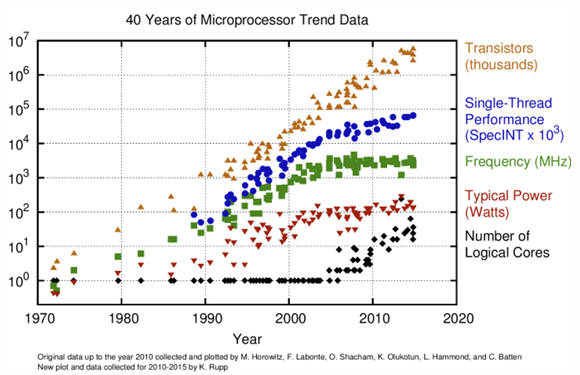
\includegraphics[width=0.49\textwidth]{figuresP/lesson_parallel_1_pag_16a.png}
    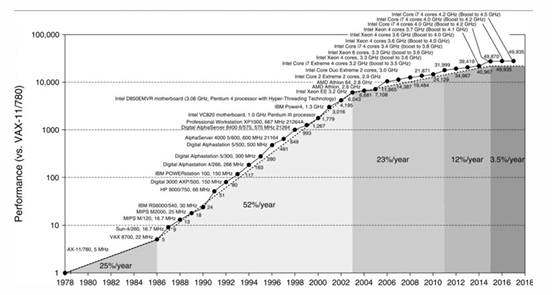
\includegraphics[width=0.49\textwidth]{figuresP/lesson_parallel_1_pag_16b.png}
\end{figure}

\subsection{Task level parallelism}

How to avoid saturation? Instruction level parallelism achieved significant performance advantages. Getting better at ILP is still possible, but the complexity of CPU is more than linear. We need a next level in parallelism: \textbf{Task Level Parallelism (TLP)}. We want our series of \textbf{instruction streams (threads) to be executed by more than one processor at once}, while at the instruction level we were talking about having a \textit{single} processor doing our work in a smarter (parallel) way. 

Let's start by introducing the so-called \textbf{Flynn's taxonomy}, which is a classification of computer architectures based on the number of data streams and instructions streams. It consists of 4 categories:
\begin{itemize}
    \item[-] Single Instruction Single Data (SISD)
    \item[-] Single Instruction Multiple Data (SIMD)
    \item[-] Multiple Instructions Single Data (MISD)
    \item[-] Multiple Instructions Multiple Data (MIMD)
\end{itemize}
Let's take a look at each of them.

In a \textbf{Single Instruction Single Data} architecture, only one instruction operates for each time slot on one data. That's the familiar sequential processing.

Example: The operations \texttt{a+b}, \texttt{c+d}, \texttt{e+f}, \texttt{g+h} will be executed one after the other.

\begin{center}
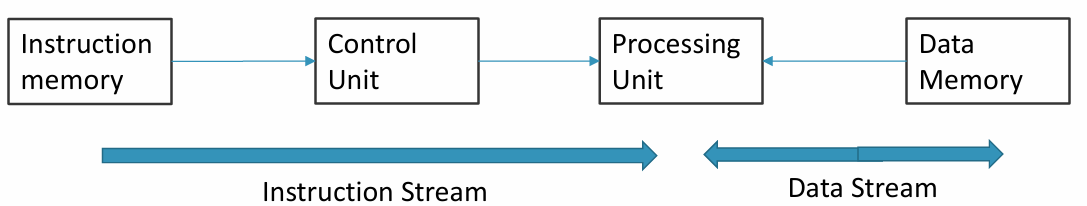
\includegraphics[width=0.7\textwidth]{figuresP/lesson_parallel_1_pag_19.png}
\end{center}

In a \textbf{Single Instruction Multiple Data} architecture, one instruction can operate on multiple data at once. Modern processors implement SIMD via vector registers, as seen in the ILP section.

Example: The operations \texttt{a+b}, \texttt{c+d}, \texttt{e+f}, \texttt{g+h} can be executed together, since it's the same instruction (the addition) that is executed on different variables. That corresponds to a vector sum.

\begin{center}
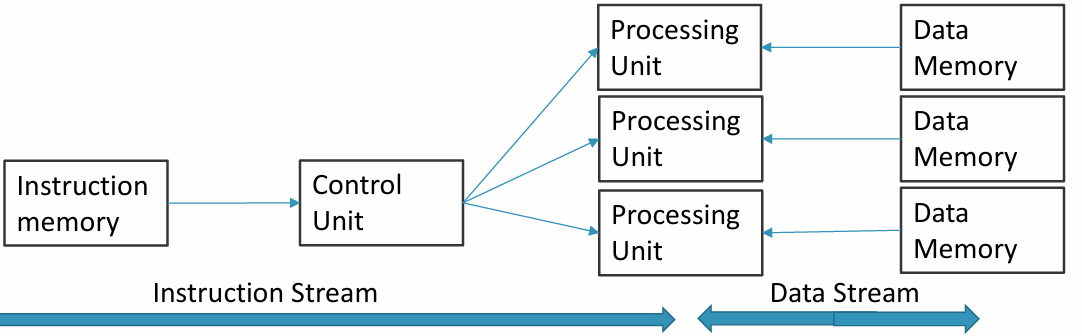
\includegraphics[width=0.7\textwidth]{figuresP/lesson_parallel_1_pag_20.png}
\end{center}

In a \textbf{Multiple Instruction Multiple Data} architecture, multiple instruction streams can operate on multiple data streams. Most supercomputers are organized as MIMD architectures including multi-core superscalar processors, multi-processor systems, and distributed systems.

Example: The operations \texttt{a+b}, \texttt{c+d}, \texttt{e*f}, \texttt{g*h} can be executed together, even if they consist of two instructions (addition and multiplication) that are executed on different variables.

\begin{center}
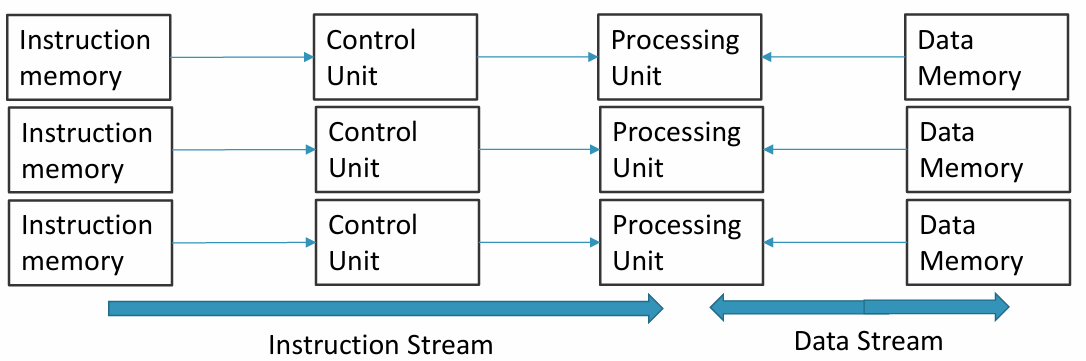
\includegraphics[width=0.7\textwidth]{figuresP/lesson_parallel_1_pag_21.png}
\end{center}

In a \textbf{Multiple Instruction Single Data} architecture, multiple instruction streams can operate on a single data stream. It is not commonly seen for computing. Sometimes the so-called \textit{systolic array} is seen as MISD (we won't treat it here). Usually, this is an architecture used for fault tolerance (processing a certain data more than once to be sure of the result), like in some pacemakers. 

\begin{center}
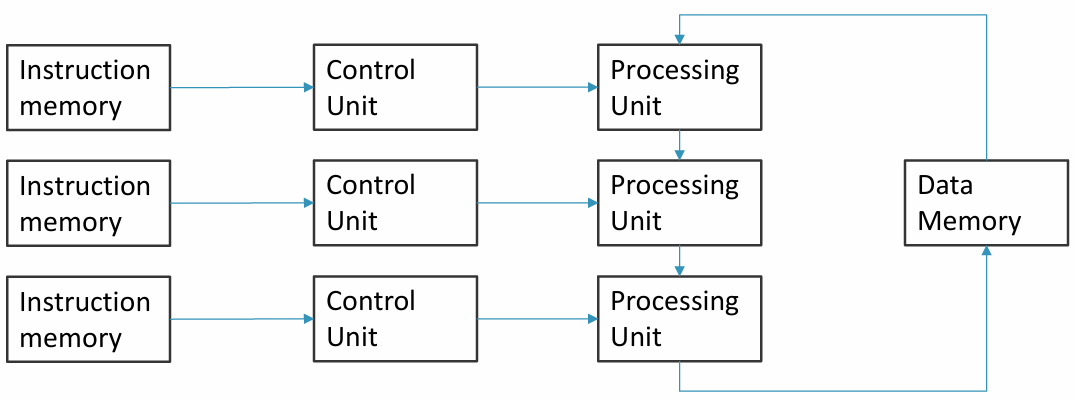
\includegraphics[width=0.7\textwidth]{figuresP/lesson_parallel_1_pag_22.png}
\end{center}

\subsection{Multiprocessors}
The standard for modern high-performance computing is the \textbf{Multiprocessor} system, an implementation of the MIMD architecture. Unlike SIMD, where a single controller drives multiple ALUs, here each processor is fully independent (it has its own PC) and communicates via \textbf{shared memory}.

We can utilize a multiprocessor system for two main goals:
\begin{itemize}
    \item \textbf{Job-level parallelism}: Running independent processes on different processors to increase throughput (e.g., browser on Core 1, compiler on Core 2). No program modification is needed.
    \item \textbf{Parallel processing}: Using multiple processors to speed up a \textit{single} program. This requires the program to be explicitly designed for parallelism using multiple cooperating threads.
\end{itemize}

To implement parallel processing, the programmer must decompose the problem into parts that can run simultaneously. There are two main approaches:

\begin{itemize}
    \item \textbf{Domain Decomposition}: The \textit{data} is divided into chunks, and parallel tasks perform the same operation on different data segments. \\
    Example: An image processing tool where the image is sliced into 4 parts, and 4 processors apply the same filter to their respective slice simultaneously. Ideally suited for both SIMD units and MIMD architectures.
    \begin{center}
    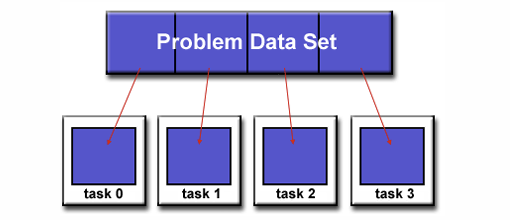
\includegraphics[width=0.38\textwidth]{figuresP/lesson_parallel_1_pag_23.png}
    \end{center}
    \item \textbf{Functional Decomposition}: The program is divided into distinct functions or tasks.\\
    Example: In a video editor, one thread handles the UI, another decodes audio, and a third renders the video preview. MIMD architectures are required here, as the processors must execute different instructions streams.
    \begin{center}
    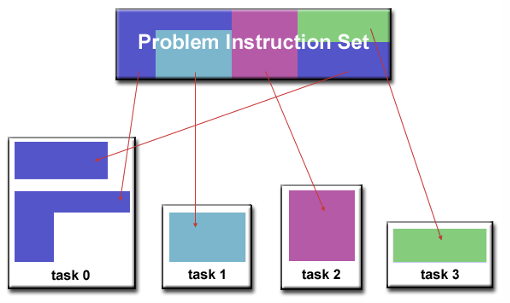
\includegraphics[width=0.38\textwidth]{figuresP/lesson_parallel_1_pag_23a.png}
    \end{center}
\end{itemize}

Now that you know what task level parallelism is, let's talk about another way to execute multiple programs: \textit{concurrency}.

\subsection{Concurrency}

As said, in a sequential processing one step follows another in sequence, and one processor is all that is needed to run the algorithm. To be more technical, you can say that each \textit{thread} of the program is executed one after the other.

Knowing what we said in this section, we expect that a computer with a single processing unit cannot do better than sequential processing. However, you might have used a single-core computer and been able to open a browser while listening to some music, for example. How is that possible? That's a first example of what is called \textbf{Concurrent Processing}.

\textbf{Concurrency} is a property of the system where multiple tasks are logically "in progress" at the same time. But wait, isn't this the definition of parallelism? Not really, we will get to it in a second.\\
There are 4 main types of concurrent processing implementation: (the first one should start to clarify the difference between parallelism and concurrency):

\subsubsection{- Multiprogramming (Time-sharing)}
In a \textbf{multiprogramming} context, a single CPU is shared among many users or programs, thanks to a time-shared algorithm or a priority algorithm. How is it possible? The CPU gives the illusion of simultaneous processing by interleaving threads with a series of \textbf{context switches}. For example, it will execute a certain thread A until a certain latency has to happen (e.g. waiting for an I/O), then with a context switch it may start to work on thread B and so on until all the tasks are executed. That's why you can listen to Gangnam Style while searching for "Best 10 moments of respect in sports" on Google in a single-core computer: you are not really running the two programs together, you are constantly switching between one and the other several times per second. 

\begin{center}
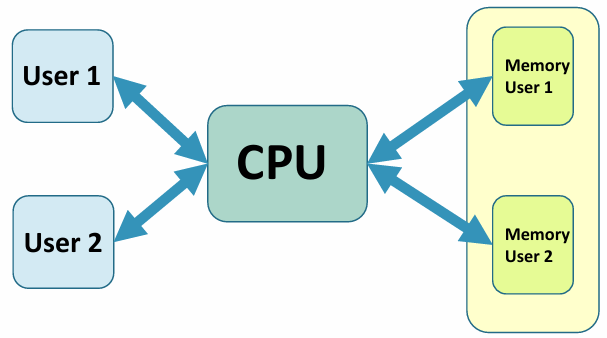
\includegraphics[width=0.4\textwidth]{figuresP/lesson_parallel_1_pag_28.png}
\end{center}

\subsubsection{- Multiprocessing (Hardware Parallelism)}
If one or more users execute multiple tasks at the same time while using multiple cores in a multiprocessor, it is referred to as \textbf{multiprocessing}. Of course this doesn't mean that every single processor can't also timeshare among several tasks. Remember that in this case the memory is shared between the cores. 

\begin{center}
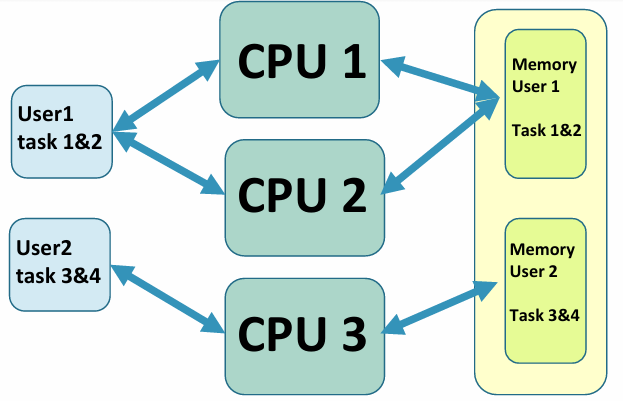
\includegraphics[width=0.4\textwidth]{figuresP/lesson_parallel_1_pag_29.png}
\end{center}

\subsubsection{- Multitasking}
We refer to \textbf{multitasking} when a single user has multiple tasks active at the same time. This is a general term from the user's perspective. It can be implemented via multiprogramming (on a single core) or true multiprocessing (on multiple cores). \\
In our example, one core plays Gangnam Style, and the other plays the heart-warming video. 

\begin{center}
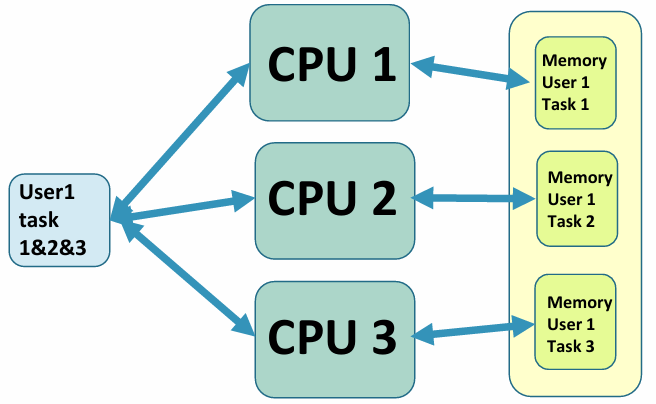
\includegraphics[width=0.4\textwidth]{figuresP/lesson_parallel_1_pag_30.png}
\end{center}

\subsubsection{- Distributed systems}
Lastly, in the so-called \textbf{distributed systems}, multiple computers even physically distant from one another can be used by the user to execute a single task. 

\begin{center}
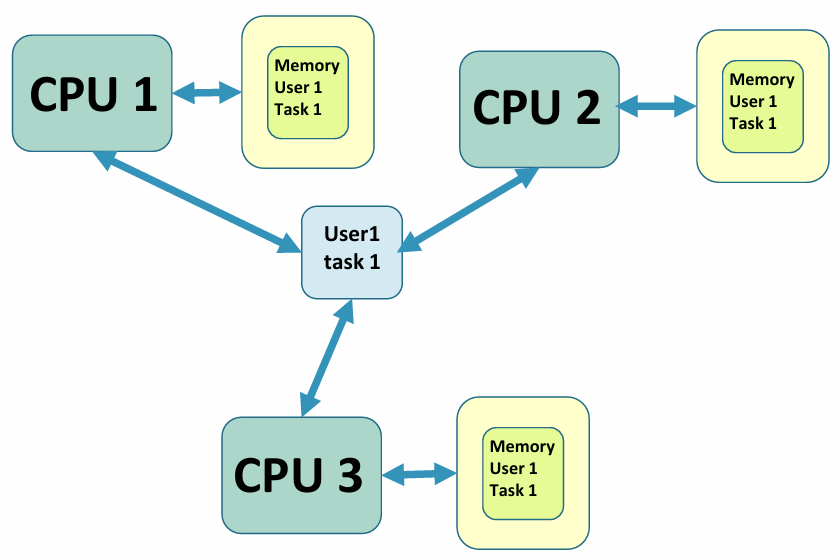
\includegraphics[width=0.4\textwidth]{figuresP/lesson_parallel_1_pag_31.png}
\end{center}

The advantages of concurrency are pretty obvious:
\begin{itemize}
    \item[-] Concurrent processes can reduce duplication;
    \item[-] The overall runtime of the algorithm can be significantly reduced;
    \item[-] More real-world problems can be solved than with sequential algorithms alone
\end{itemize}
However there are also many disadvantages:
\begin{itemize}
    \item[-] Runtime is not always reduced, so careful planning is required;
    \item[-] Concurrent algorithms can be more complex than sequential algorithms;
    \item[-] Shared data can be corrupted;
    \item[-] Communication between tasks is needed.
\end{itemize}

With that said, \textbf{what's the difference between concurrency and parallelization?} Concurrency is the execution of multiple tasks at the same time, regardless of the number of processors. Parallelism is the execution on multiple processors of the same task, which consists in breaking the task into meaningful pieces, doing the work on many processors, coordinating and putting the pieces back together.\\
More specifically, \textbf{concurrency is a property of the program structure}: it means dealing with multiple things at once (managing multiple start/end times). \textbf{Parallelism is a property of the machine execution}: it means doing multiple things at the exact same instant. A system can be concurrent without being parallel (e.g. multitasking on a single core via time-slicing) and can be parallel (e.g. bit-level instructions) without being concurrent. However, in high performance computing,\textit{ we typically aim for concurrency executed via parallelism to achieve maximum speed}. For example, imagine you have to render a 10-second video clip consisting of 300 frames.
\begin{itemize}
    \item[-] Concurrency (The Logic): The video editing software is designed to treat each frame as an independent task. The program creates 300 threads, one for each frame. This is concurrency: the structure allows multiple things to happen.
    \item[-] Parallelism (The Hardware): If you run this on a generic single-core laptop, the CPU will switch rapidly between frames (concurrency without parallelism). If you run this on a 16-core workstation, the CPU physically renders 16 frames at the exact same instant. This is concurrency executed via parallelism, resulting in a massive reduction of total execution time.
\end{itemize}

\subsection{Characteristics of task-level parallelization}
For a wide class of algorithms parallelization is the most powerful way to decrease execution time (not its complexity). For example, in a problem with $O(N\log N)$ complexity (e.g. quicksort) on $\log N$ processors should take the time needed by $O(N)$ algorithms. Or a problem with $O(N^2)$ complexity (e.g. bubble search) on N processors should take the time needed by $O(N)$ algorithms. As we will soon see, this is an oversimplified and (most of the time) wrong reasoning.

Parallelization is not free. Processors must be controlled and coordinated, i.e. we need a way to govern which processor does what work. The program must often be written in a special programming language for parallel systems and a parallelized program for one machine (with, say, 2K processors) might not be optimal on other machines (with, say, 2L processors).

Let's start by asking the most simple question: how much time can we gain from parallelizing an algorithm?
We define the \textbf{speed-up} as 
\begin{equation*}
    S_{n}=T_{s}  \ / \ T_{p}(n)    
\end{equation*}
where $T_{s}$ is the time needed to execute a task with a serial execution and $T_{p}(n)$ is the time needed to execute the same task with a parallel execution on $n$ processors. 
For a perfect parallel algorithm $S_{n}=n$. The vast majority of times, that is practically impossible, even if in very specific cases one could also have $S_{n}>n$ (\textit{superlinear case}).

With that in mind, we can also define the \textbf{efficiency} as 
\begin{equation*}
    E=S_{n}/n
\end{equation*}
It is a measure of how well our algorithm is using the processors. \\
Lastly, the \textbf{cost} is defined as
\begin{equation*}
    c=nT_{p}(n)=\frac{T_{1}}{E}
\end{equation*}
If we want to implement a certain algorithm using parallel processing, we also need to think about its \textbf{scalability}, which is the capability to remain efficient with an increasing number of processors.

Now that we have introduced some useful theoretical definitions, let's look at what happens in practice. What are the primary difficulties in implementing parallelization?
\begin{itemize}
    \item[-] \textbf{Load balancing}: In case of several tasks in parallel, the execution time of each task should be similar, otherwise the total time is dominated by the slower task. It's not easy to design a priori a parallel process with good load balancing, considering for instance that some of the available processors could be less efficient than others.
    \item[-] \textbf{Synchronization}: If the tasks use the same shared memory a logic of lock-unlock must be designed and the mechanism can involve a big latency
    \item[-] \textbf{Communication latency}: If data must be moved between processors, or most commonly between processors and memory, the overhead due to data transmission can be really relevant, to the point that it could make your parallel execution slower than a sequential one.
\end{itemize}
Moreover, \textit{Amdahl's law} (1967) shows one more big problem with parallelization. 

\subsection{Amdahl's law}
To easily understand the following concepts consider this example. You need to distribute 10000 flyers across the city and you have 11 workers at the office to help you. One of them has to go to the copy shop to get the 10000 flyers and the others need to distribute them. The first one does his job in an hour, the others take 1000 flyers each and in 6 hours they are done, for a total of 7 hours. How can you speed up this process? If you double the amount of workers that distribute flyers then the same job can be done in 4 hours (1+3). However, it doesn't make sense to send more than one person to get the flyers, since the time needed to reach the copy shop and come back would still be of 1 hour. That means that even with an infinite amount of workers, this job requires at least 1 hour to be completed.

This example shows us one fundamental idea: \textbf{not every part of a problem can be parallelized}. In fact, a problem that can be fully parallelized cannot exist. 

If only one part $(P_{K})$ of the problem can be improved, the maximum speed-up is given by:
\begin{equation*}
    S=1/\sum\frac{P_{K}}{S_{k}}    
\end{equation*}
where $k$ is the part of the problem and $S_{k}$ is the speed-up of $k$. That's \textbf{Amdahl's law}, which can be applied to every kind of problem. \\
In the case of parallel programming:
\begin{equation*}
    S_{n}=\frac{n}{na+(1-a)}    
\end{equation*}
where $a$ is the fraction of the code that cannot be parallelized.
If $n\rightarrow\infty$ the speed-up is $S_{n}=\frac{1}{a}$. Take a look at the image below. If the fraction of serial code is 10\% ($a=0.10$) the maximum speed-up is only 10 \textbf{regardless of the number of processors}. Even with tens of thousands of processors the results are scarce (for reference a 10x speed-up can be obtained just with a deep pipeline). 

\begin{center}
    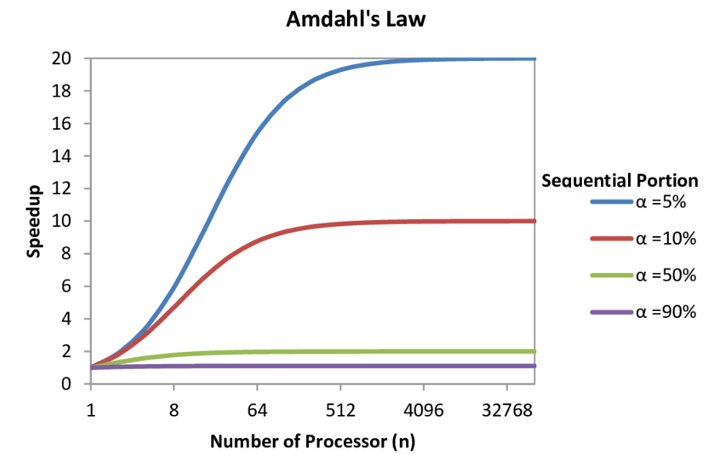
\includegraphics[width=0.6\textwidth]{figuresP/lesson_parallel_1_pag_36.png}
\end{center}

So apparently parallelism is useful only for "embarrassingly parallel" problems, with a small number of processors. Why bother, then?

Fortunately, there are important caveats to this law. One in particular is the key to solve all of our doubts on the usefulness of parallelism: Amdahl assumes that the dimension of the problem is always the same when increasing the number of processors, \textbf{but more processors means that wider problems can be addressed}. It's intuitive, but not trivial. 

In our example having 1000 workers is an obvious overkill if there are only 10000 flyers. However, with 1000 workers you could distribute a million flyers in 7 hours. The same thing goes with processors: 2 CPUs could easily compute the product of two $4\times4$ matrices, but for $1000\times1000$ matrices you are in need of much more processing power. 

In other words, Amdahl's law assumes that the \textit{scale} of the problem is fixed, which is absolutely not the case in the most useful applications of parallelism.

Lastly, Amdahl also assumes that the best solution is always the best serial algorithm but some problems require to be solved in parallel by their very nature. 

\subsection{Gustafson's law}
Let's define $t_s$ as the time of the serial part and $t_p$ as the time of the  parallel part. Now we take a problem that grows with the number of processors $n$ while the serial part remains always the same (e.g. when the number of flyers doubles, the number of workers does too). Under these assumptions, \textbf{Gustafson's law} (1988) tells us that the speed-up is given by:
\begin{equation*}
    S_{n}=n+(1-n)s 
\end{equation*}
That means that $S_n\propto n$, just like shown in the following figure.

\begin{center}
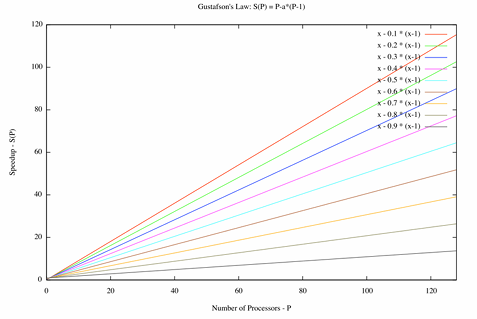
\includegraphics[width=0.5\textwidth]{figuresP/lesson_parallel_1_pag_39.png}
\end{center}

This last figure compares Amdahl's and Gustafson's law, showcasing how the speed-up changes when one assumes a fixed problem size or a fixed execution time respectively.

\begin{center}
    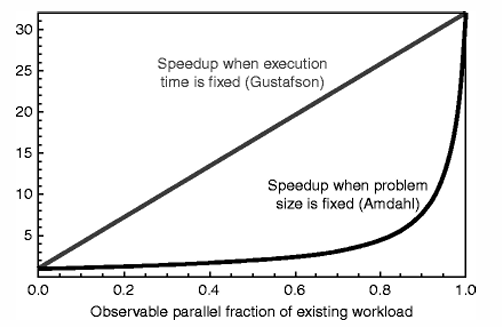
\includegraphics[width=0.5\textwidth]{figuresP/lesson_parallel_1_pag_39a.png}
\end{center}






